\fenicschapter{Computational Thermodynamics}
              {Computational Thermodynamics}
              {Johan~Hoffman, Claes~Johnson and Murtazo Nazarov} 

\editornote{Missing figures, need to be added in EPS sub directory.}
\editornote{Missing bibliography, needs to be added to common bibliography.bib in correct format.}

We test the functionality of FEniCS on the challenge of computational
thermodynamics in the form of a finite element solver of the Euler
equations expressing conservation of mass, momentum and energy. We
show that computational solutions satisfy a 2nd Law formulated in
terms of kinetic energy, internal (heat) energy, work and
shock/turbulent dissipation, without reference to entropy. We show
that the 2nd Law
%The Euler equations
%are regularized in computational solution 
%by a least-squares stabilized finite element method referred
%to as EG2. The 2nd Law expresses 
expresses an irreversible transfer of kinetic energy to heat energy in
shock/turbulent dissipation arising because the Euler equations lack
pointwise solutions, and thus explains the occurence of
irreversibility in formally reversible systems as an effect of
instability with blow-up of Euler residuals combined with finite
precision computation, without resort to statistical mechanics or ad
hoc viscous regularization.
%EG2 includes a duality-based posteriori error control showing that mean-value outputs can be 
%computable to tolerances of interest. 
We simulate the classical Joule experiment of a gas expanding from
rest under temperature drop followed by temperature recovery by
turbulent dissipation until rest in the double volume.
 
\section{FEniCS as Computational Science}

The goal of the FEniCS project is to develop software for automated
computational solution of differential equations based on a finite
element methodology combining generality with efficiency. The FEniCS
Application Unicorn offers a solver for a fluid-solids continuum based
on a unified Eulerian formulation of momentum balance combined with
constitutive laws for fluid/solid in Eulerian/updated Lagrangian form,
which shows the capability of FEniCS for automation of computational
fluid-structure interaction.

Thermodynamics is a basic area of continuum mechanics with many
important applications, which however is feared by both teachers,
students and engineers as being difficult to understand and to apply,
principally because of the apperance of turbulence. In this article we
show that turbulent thermodynamics can be made understandable and
useful by automated computational solution, as another example of the
capability of FEniCS.

The biggest mystery of classical thermodynamics is the 2nd Law about
entropy and automation cannot harbor any mystery.  Expert systems are
required for mysteries and FEniCS is not an expert system.  Automation
requires a continuum mechanics formulation of thermodynamics with a
transparent 2nd Law.  We present a formulation of thermodynamics based
on finite precision computation with a 2nd Law without reference to
entropy, which we show can serve as a basis for automated
computational simulation of complex turbulent thermodynamics and thus
can open to new insight and design, a main goal of FEniCS. In this
setting the digital finite element model becomes the real model of the
physics of thermodynamics viewed as a form of analog finite precision
computation, a model which is open to inspection and analysis because
solutions can be computed and put on the table. This represents a new
kind of science in the spirit of Dijkstra \cite{dijkstra} and Wolfram
\cite{wolfram}, which can be explored using FEniCS and which we
present in non-technical form in My Book of Knols \cite{knol}.

\section{The 1st and 2nd Laws of Thermodynamics}

\small
\begin{quote} Heat, a quantity which functions to animate, derives
from an internal fire located in the left ventricle. (Hippocrates, 460 B.C.)
\end{quote}
\small
\normalsize

\emph{Thermodynamics} is fundamental in a wide range of phenomena from
macroscopic to microscopic scales.  Thermodynamics essentially
concerns the interplay between \emph{heat energy} and \emph{kinetic
energy} in a \emph{gas} or \emph{fluid}.  Kinetic energy, or
\emph{mechanical energy}, may generate heat energy by
\emph{compression} or \emph{turbulent dissipation}.  Heat energy may
generate kinetic energy by \emph{expansion}, but not through a
\emph{reverse} process of turbulent dissipation.  The industrial
society of the 19th century was built on the use of \emph{steam
engines}, and the initial motivation to understand thermodynamics came
from a need to increase the efficiency of steam engines for conversion
of heat energy to useful mechanical energy.  Thermodynamics is closely
connected to the dynamics of \emph{slightly viscous} and
\emph{compressible} gases, since substantial compression and expansion
can occur in a gas, but less in fluids (and solids).

The development of classical thermodynamics as a rational science
based on logical deduction from a set of axioms, was initiated in the
19th century by Carnot \cite{carnot}, Clausius \cite{clausius} and
Lord Kelvin \cite{kelvin}, who formulated the basic axioms in the form
of the \emph{1st Law} and the \emph{2nd Law} of thermodynamics. The
1st Law states (for an isolated system) that the \emph{total energy},
the sum of kinetic and heat energy, is conserved.  The 1st Law is
naturally generalized to include also conservation of mass and
Newton's law of conservation of momentum and then can be expressed as
the \emph{Euler equations} for a gas/fluid with \emph{vanishing
viscosity}.
%The 1st law can be viewed as a definition, with any loss of kinetic 
%energy defined to be heat energy. 

The 2nd Law has the form of an inequality $dS\ge 0$ for a quantity
named \emph{entropy} denoted by $S$, with $dS$ denoting change
thereof, supposedly expressing a basic feature of real thermodynamic
processes.  The classical 2nd Law states that the entropy cannot
decrease; it may stay constant or it may increase, but it can never
decrease (for an isolated system).

The role of the 2nd Law is to give a scientific basis to the many
observations of \emph{irreversible} processes, that is, processes
which cannot be reversed in time, like running a movie backwards.
Time reversal of a process with strictly increasing entropy, would
correspond to a process with strictly decreasing entropy, which would
violate the 2nd Law and therefore could not occur. A perpetum mobile
would represent a reversible process and so the role of the 2nd Law is
in particular to explain \emph{why} it is imposssible to construct a
perpetum mobile, and \emph{why} time is moving forward in the
direction an \emph{arrow of time}, as expressed by Max Planck
\cite{planck1,planck2,planck3}: \emph{Were it not for the existence of
irreversible processes, the entire edifice of the 2nd Law would
crumble}.

While the 1st Law in the form of the Euler equations expressing
conservation of mass, momentum and total energy can be understood and
motivated on rational grounds, the nature of the 2nd Law is
mysterious.  It does not seem to be a consequence of the 1st Law,
since the Euler equations seem to be time reversible, and the role of
the 2nd Law is to explain irreversibility. Thus questions are lining
up: nIf the 2nd Law is a new independent law of Nature, how can it be
justified? What is the physical significance of that quantity named
entropy, which Nature can only get more of and never can get rid of,
like a steadily accumulating heap of waste? What mechanism prevents
Nature from recycling entropy? How can irreversiblity arise in a
reversible system? How can viscous dissipation arise in a system with
vanishing viscosity? Why is there no \emph{Maxwell demon}
\cite{maxwell}?  Why can a gas by itself expand into a larger volume,
but not by itself contract back again, if the motion of the gas
molecules is governed by the reversible Newton's laws of motion? Why
is there an arrow of time? This article presents answers.

%\begin{figure}[bhpt] 
%\centerline{ 
%\includegraphics[height=12.0cm]{ambsthermopict/newcdiag.eps} 
%} 
%\caption{Converting heat to kinetic (mechanical) energy in 1712.}
%\label{nse_people} 
%\end{figure}

\section{The Enigma}
\small
\begin{quote}
Those who have talked of ``chance'' are the
inheritors of antique superstition and ignorance...whose minds have never
been illuminated by a ray of scientific thought. (T. H. Huxley)
\end{quote}
\normalsize

These were the questions which confronted scientists in the late 19th
century, after the introduction of the concept of entropy by Clausius
in 1865, and these showed to be tough questions to answer.  After much
struggle, agony and debate, the agreement of the physics community has
become to view \emph{statistical mechanics} based on an assumption of
\emph{molecular chaos} as developed by Boltzmann \cite{boltzmann}, to
offer a rationalization of the classical 2nd Law in the form of a
tendency of (isolated) physical processes to move from improbable
towards more probable states, or from ordered to less ordered states.
Boltzmann's assumption of molecular chaos in a dilute gas of colliding
molecules, is that two molecules about to collide have independent
velocities, which led to the \emph{H-theorem} for \emph{Boltzmann's
equations} stating that a certain quantity denoted by $H$ could not
decrease and thus could serve as an entropy defining an arrow of time.
Increasing disorder would thus represent increasing entropy, and the
classical 2nd Law would reflect the eternal pessimistists idea that
things always get more messy, and that there is really no limit to
this, except when everything is as messy as it can ever get. Of
course, experience could give (some) support this idea, but the
trouble is that it prevents things from ever becoming less messy or
more structured, and thus may seem a bit too pessimistic.  No doubt,
it would seem to contradict the many observations of \emph{emergence}
of ordered non-organic structures (like crystals or waves and cyclons)
and organic structures (like DNA and human beings), seemingly out of
disordered chaos, as evidenced by the physics Nobel Laureate Robert
Laughlin \cite{laughlin}.

%\begin{figure}[bhpt] 
%\centerline{ 
%\includegraphics[height=6.0cm]{ambsthermopict/lawsofthermodynamics.eps} 
%} 
%\caption{Classical thermodynamics in a nutshell (from the web).}
%\label{nse_people} 
%\end{figure}

Most trained thermodynamicists would here say that emergence of order
out of chaos, in fact does not contradict the classical 2nd Law,
because it concerns ``non-isolated systems''. But they would probably
insist that the Universe as a whole (isolated system) would steadily
evolve towards a ``heat-death'' with maximal entropy/disorder (and no
life), thus fulfilling the pessimists expectation. The question from
where the initial order came from, would however be left open.

The standard presentation of thermodynamics based on the 1st and 2nd
Laws, thus involves a mixture of deterministic models (Boltzmann's
equations with the H-theorem) based on statistical assumptions
(molecular chaos) making the subject admittedly difficult to both
learn, teach and apply, despite its strong importance. This is
primarily because the question \emph{why} necessarily $dS\ge 0$ and
never $dS<0$, is not given a convincing understandable answer.  In
fact, statistical mechanics allows $dS<0$, although it is claimed to
be very unlikely. The basic objective of statistical mechanics as the
basis of classical thermodynamics, thus is to (i) give the entropy a
physical meaning, and (ii) to motivate its tendency to (usually)
increase. Before statistical mechanics, the 2nd Law was viewed as an
experimental fact, which could not be rationalized theoretically. The
classical view on the 2nd Law is thus either as a statistical law of
large numbers or as a an experimental fact, both without a rational
deterministic mechanistic theoretical foundation. The problem with
thermodynamics in this form is that it is understood by very few, if
any:

\small
\begin{itemize}
\item \emph{Every mathematician knows it is impossible to understand
an elementary course in thermodynamics.} (V. Arnold)
\item \emph{...no one knows what entropy is, so if you in a debate use
this concept, you will always have an advantage.} (von Neumann to
Shannon)
\item \emph{As anyone who has taken a course in thermodynamics is well
aware, the mathematics used in proving Clausius' theorem (the 2nd Law)
is of a very special kind, having only the most tenous relation to
that known to mathematicians.} (S. Brush \cite{brush})
\item \emph{Where does irreversibility come from? It does not come
form Newton's laws. Obviously there must be some law, some obscure but
fundamental equation. perhaps in electricty, maybe in neutrino
physics, in which it does matter which way time goes.} (Feynman
\cite{feynman})
\item
\emph{For three hundred years science has been dominated by a
Newtonian paradigm presenting the World either as a sterile mechanical
clock or in a state of degeneration and increasing disorder...It has
always seemed paradoxical that a theory based on Newtonian mechanics
can lead to chaos just because the number of particles is large, and
it is subjectivly decided that their precise motion cannot be observed
by humans... In the Newtonian world of necessity, there is no arrow of
time. Boltzmann found an arrow hidden in Nature's molecular game of
roulette.}  (Paul Davies \cite{davies})
\item \emph{The goal of deriving the law of entropy increase
from statistical mechanics has so far eluded the deepest
thinkers.} (Lieb \cite{lieb})
\item \emph{There are great physicists who have not understood it}.
(Einstein about Boltzmann's statistical mechanics) 
\end{itemize}
\normalsize
 
\section{Computational Foundation}   

In this note we present a foundation of thermodynmaics, further
elaborated in \cite{hoffman,ambsthermo}, where the basic assumption of
statistical mechanics of molecular chaos, is replaced by
\emph{deterministic finite precision computation}, more precisely by a
\emph{least squares stabilized finite element method} for the Euler
equations, referred to as \emph{Euler General Galerkin} or \emph{EG2}.
In the spirit of Dijkstra \cite{dijkstra}, we thus view EG2 as the
physical model of thermodynamics, that is the Euler equations together
with a computational solution procedure, and not just the Euler
equations without constructive solution procedure as in a classical
non-computational approach.

Using EG2 as a model of thermodynamics changes the questions and
answers and opens new possibilities of progress together with new
challenges to mathematical analysis and computation.  The basic new
feature is that EG2 solutions are computed and thus are available to
inspection. This means that the analysis of solutions shifts from
\emph{a priori} to \emph{a posteriori}; after the solution has been
computed it can be inspected.

Inspecting computed EG2 solutions we find that they are
\emph{turbulent} and have \emph{shocks}, which is identified by
pointwise large Euler residuals, reflecting that pointwise solutions
to the Euler equations are lacking. The enigma of thermodynamics is
thus the enigma of turbulence (since the basic nature of shocks is
understood). Computational thermodynamics thus essentially concerns
computational turbulence. In this note and \cite{ambsthermo} we
present evidence that EG2 opens to a resolution of the enigma of
turbulence and thus of thermodynamics.
 
The fundamental question concerns \emph{wellposedness} in the sense of
Hadamard, that is what aspects or \emph{outputs} of turbulent/shock
solutions are stable under perturbations in the sense that small
perturbations have small effects. We show that wellposedness of EG2
solutions can be tested a posteriori by computationally solving a
\emph{dual linearized problem}, through which the output sensitivity
of non-zero Euler residuals can be estimated. We find that mean-value
outputs such as drag and lift and total turbulent dissipation are
wellposed, while point-values of turbulent flow are not. We can thus a
posteriori in a case by case manner, assess the quality of EG2
solutions as solutions of the Euler equations.
%But we refrain from the seemingly hopeless task of proving a 
%priori that EG2 will produce wellposed solutions for all data.    

We formulate a \emph{2nd Law} for EG2 
without the concept of entropy, in terms of  
the basic physical quantities of kinetic energy
$K$, heat energy $E$, rate of \emph{work} $W$ and shock/turbulent dissipation
$D>0$. The new 2nd Law reads
\begin{equation}\label{secondlaw}
\dot K=W-D,\quad \dot E=-W+D,
\end{equation}
where the dot indicates time differentiation. Slightly viscous
flow always develops turbulence/shocks with $D>0$, and the  
2nd Law thus expresses an irreversible transfer of kinetic energy
into heat energy, while the total energy $E+K$ remains constant.

With the 2nd Law in the form (\ref{secondlaw}), we avoid the
(difficult) main task of statistical mechanics of specifying the
physical significance of entropy and motivating its tendency to
increase by probabilistic considerations based on (tricky)
combinatorics. Thus using \emph{Ockham's razor} \cite{ockham}, we
rationalize a scientific theory of major importance making it both
more understandable and more useful. The new 2nd Law is closer to
classical Newtonian mechanics than the 2nd Law of statistical
mechanics, and thus can be viewed to be more fundamental.

The new 2nd Law is a consequence of the 1st Law in the form of the
Euler equations combined with EG2 finite precision computation
effectively introducing viscosity and viscous dissipation. These
effects appear as a consequence of the non-existence of pointwise
solutions to the Euler equations reflecting instablities leading to
the development shocks and turbulence in which large scale kinetic
energy is transferred to small scale kinetic energy in the form of
heat energy. The viscous dissipation can be interpreted as a penalty
on pointwise large Euler residuals arising in shocks/turbulence, with
the penalty being directly coupled to the violation following a
principle of criminal law exposed in \cite{foucault}.  EG2 thus
explains the 2nd Law as a consequence of the non-existence of
pointwise solutions with small Euler residuals.  This offers an
understanding to the emergence of irreversible solutions of the
formally reversible Euler equations.  If pointwise solutions had
existed, they would have been reversible without dissipation, but they
don't exist, and the existing computational solutions have dissipation
and thus are irreversible.

\section{Viscosity Solutions}

An EG2 solution can be viewed as particular \emph{viscosity solution}
of the Euler equations, which is a solution of \emph{regularized Euler
equations} augmented by additive terms modeling viscosity effects with
small viscosity coefficients. The effective viscosity in an EG2
solution typically may be comparable to the mesh size.

For incompressible flow the existence of viscosity solutions, with
suitable solution dependent viscosity coefficients, can be proved a
priori using standard techniques of analytical mathematics.  Viscosity
solutions are pointwise solutions of the regularized equations.  But
already the most basic problem with constant viscosity, the
incompressible Navier-Stokes equations for a Newtonian fluid, presents
technical difficulties, and is one of the open Clay Millennium
Problems.

For compressible flow the technical complications are even more
severe, and it is not clear which viscosities would be required for an
analytical proof of the existence of viscosity solutions
\cite{feireisl} to the Euler equations.  Furthermore, the question of
wellposedness is typically left out, as in the formulation of the
Navier-Stokes Millennium Problem, with the motivation that first the
existence problem has to be settled.  Altogether, analytical
mathematics seems to have little to offer a priori concerning the
existence and wellposedness of solutions of the compressible Euler
equations.  In contrast, EG2 computational solutions of the Euler
equations seem to offer a wealth of information a posteriori, in
particular concerning wellposedness by duality.

An EG2 solution thus can be viewed as a specific viscosity solution
with a specific regularization from the least squares stabilization,
in particular of the momentum equation, which is necessary because
pointwise momentum balance is impossible to achieve in the presence of
shocks/turbulence.  The EG2 viscosity can be viewed to be the minimal
viscosity required to handle the contradiction behind the
non-existence of pointwise solutions.  For a shock EG2 could then be
directly interpreted as a certain physical mechanism preventing a
shock wave from turning over, and for turbulence as a form of
automatic computational turbulence model.

EG2 thermodynamics can be viewed as form of deterministic chaos, where
the mechanism is open to inspection and can be used for prediction. On
the other hand, the mechanism of statistical mechanics is not open to
inspection and can only be based on ad hoc assumption, as noted by
e.g. Einstein \cite{einsteincit1}. If Boltzmann's assumption of
molecular chaos cannot be justified, and is not needed, why consider
it at all, \cite{loschmidt}?

\begin{figure}[bhpt] 
\centerline{ 
%\includegraphics[height=6cm]{fig358.eps} 
} 
\caption{Joule's 1845 experiment}
\label{joule} 
\end{figure} 

\editornote{Missing figure.}

\section{Joule's 1845 Experiment} 

To illustrate basic aspects of thermodynamics, we recall Joule's
experiment from 1845 with a gas initially at rest with temperature $T
=1$ at a certain pressure in a certain volume immersed into a
container of water, see Fig. \ref{joule}. At initial time a valve was
opened and the gas was allowed to expand into the double volume while
the temperature change in the water was carefully measured by Joule.
To the great surprise of both Joule and the scientific community, no
change of the temperature of the water could be detected, in
contradiction with the expectation that the gas would cool off under
expansion.  Moreover, the expansion was impossible to reverse; the gas
had no inclination to contract back to the original volume.
Simulating Joule's experiment using EG2, we discover the following as
displayed in Fig. \ref{joule_den}-\ref{joule_kin2}

\begin{figure}[bhpt] 
\centerline{ 
%\includegraphics[height=3.5cm]
%{ambsthermopict/joule-pics/joule-chamber-den-1.eps} 
%\includegraphics[height=3.5cm]
%{ambsthermopict/joule-pics/joule-chamber-den-2.eps} 
} 
\caption{Density at two time instants}
\label{joule_den} 
\end{figure}
\begin{figure}[bhpt] 
\centerline{ 
%\includegraphics[height=3.5cm]
%{ambsthermopict/joule-pics/joule-chamber-tem-1.eps} 
%\includegraphics[height=3.5cm]
%{ambsthermopict/joule-pics/joule-chamber-tem-2.eps} 
} 
\caption{Temperature at two time instants}
\label{joule_tem} 
\end{figure}

\begin{figure}[bhpt] 
\centerline{ 
%\includegraphics[height=2.0cm]
%{ambsthermopict/joule-pics/joule-den-lc.eps}
%\includegraphics[height=2.0cm]
%{ambsthermopict/joule-pics/joule-den-rc.eps}
} 
\caption{Average density in left and right chamber}
\label{joule_den2} 
\end{figure}

\begin{figure}[bhpt] 
\centerline{ 
%\includegraphics[height=2.0cm]
%{ambsthermopict/joule-pics/joule-tem-lc.eps}
%\includegraphics[height=2.0cm]
%{ambsthermopict/joule-pics/joule-tem-rc.eps} 
} 
\caption{Average temperature in left and right chamber}
\label{joule_tem2} 
\end{figure}

\begin{figure}[bhpt] 
\centerline{ 
%\includegraphics[height=2.0cm]
%{ambsthermopict/joule-pics/joule-chamber-kinene-1.eps} 
%\includegraphics[height=2.0cm]
%{ambsthermopict/joule-pics/joule-chamber-temp.eps} 
} 
\caption{Average kinetic energy and temperature: short time}
\label{joule_kin} 
\end{figure}
\begin{figure}[bhpt] 
\centerline{
%\includegraphics[height=3.0cm]
%{ambsthermopict/joule-pics/joule-kinene-1.eps} 
%\includegraphics[height=3.0cm]
%{ambsthermopict/joule-pics/joule-kin-lc.eps}   
%\includegraphics[height=3.0cm]
%{ambsthermopict/joule-pics/joule-kin-rc.eps} 
} 
\caption{Average kinetic energy in both, left and right chamber(s): long time}
\label{joule_kin2} 
\end{figure}

In a first phase the temperature drops below 1 as the gas expands with
increasing velocity, and in a second phase shocks/turbulence appear
and heat the gas towards a final state with the gas at rest in the
double volume and the temperature back to $T =1$.  The total (heat)
energy is, of course, conserved since the density is reduced by a
factor 2 after expansion to double volume. We can also understand that
the rapidity of the expansion process makes it difficult to detect any
temperature drop in the water in the inital phase. Altogether, using
EG2 we can first simulate and then understand Joule's experiment, and
we thus see no reason to be surprised. We shall see below as a
consequence of the 2nd Law that reversal of the process with the gas
contracting back to the original small volume, is impossible because
the only way the gas can be put into motion is by expansion, and thus
contraction is impossible.

In statistical mechanics the dynamics of the process would be
dismissed and only the initial and final state would be subject to
analysis. The final state would then be viewed as being ``less
ordered'' or ``more probable'' or having ``higher entropy'', because
the gas would occupy a larger volume, and the reverse process with the
gas contracting back to the initial small volume, if not completely
impossible, would be ``improbable''. But to say that a probable state
is is more probable than an improbable state is more mystifying than
informative. Taking the true dynamics of the process into account
including in particular the second phase with heat generation from
shocks or turbulence, we can understand the observation of constant
temperature and irreversibility in a deterministic fashion without
using any mystics of entropy based on mystics of statistics. In
\cite{arrow} we develop a variety of aspects of the arrow of time
enforced by the new 2nd Law.

%\cite{einsteincit1,
%einsteincit2,einsteincit3}.

%\section{Limitations of Classical Thermodynamics}

%Classical thermodynamics developed in the late 19th century
%seeks to describe systems in \emph{thermodynamic equilibrium}, 
%neglecting the dynamic process
%from one equilibrium state to another with the motivation that 
%the dynamics is too complex. To describe systems in thermodynamic equilibrium
%different forms of \emph{statistical mechanics} were pioneered  
%by in particular Gibbs and Boltzmann.

%The classical formulations of the 2nd Law
%are cryptic, and thus have no clear scientific meaning. Yet the 2nd Law
%is considered as a foundation of classical thermodynamics.

%\section{Carnot Engine}
%Carnot created an equation he employed to prove this statement, and 
%currently used to show the thermodynamic efficiency of a heat machine: 
%e = 1 - TL / TH (the efficiency of a heat machine is equal to one minus 
%the low operating temperature of the machine in degrees Kelvin, divided 
%by the high operating temperate of the machine in degrees Kelvin). For a 
%machine to attain full efficiency, temperatures of absolute zero would 
%have to be incorporated.

%\small
%\begin{quote} 
%The total energy of the universe is constant; the total entropy is 
%continually increasing. (Rudolf Clausius 1865)
%\end{quote}
%\begin{quote} Everyone knows that heat can produce motion. That it possesses
%vast motive power no one can doubt, in these days when the steem engine is 
%everywhere so well known. The study of these enegines is of great interest,
%their importance is enormous, their use is contnually increasing, and they
%seem desined to produce a great revolution in the civilized world.
%(Carnot \cite{carnot} 1824).
%\end{quote}
%\begin{quote}...the whole procedure was an act of despair because a
%theoretical interpretation had to be found at any price, no matter
%how high that might be... (Planck on the statistical mechanics basis of 
%his radiation law)
%\end{quote}
%\begin{quote} Where does irreversibility come from? It does not come
%form Newton's laws. Obviously there must be some law, some
%obscure but fundamental equation. perhaps in electricty,
%maybe in neutrino physics, in which it \emph{does}
%matter which way time goes. (The Feynmman Lectures on Physics 1963)
%\end{quote}
%\begin{quote} The 2nd Law cannot be derived from purely mechanical
%laws. It carries the stamp of the essentially statitical nature of heat.
%(Bergman in Basic Theories of Physics 1951)
%\end{quote}

\section{The Euler Equations}

\small
%\begin{quote} 
%The total energy of the universe is constant; the total entropy is 
%continually increasing. (Rudolf Clausius 1865)
%\end{quote}
%\begin{quote} Everyone knows that heat can produce motion. That it possesses
%vast motive power no one can doubt, in these days when the steam engine is 
%everywhere so well known. The study of these engines is of great interest,
%their importance is enormous, their use is continually increasing, and they
%seem desined to produce a great revolution in the civilized world.
%(Carnot \cite{carnot} 1824).
%\end{quote}
%\begin{quote}...the whole procedure was an act of despair because a
%theoretical interpretation had to be found at any price, no matter
%how high that might be... (Planck on the statistical mechanics basis of 
%his radiation law)
%\end{quote}
%\begin{quote} The 2nd Law cannot be derived from purely mechanical
%laws. It carries the stamp of the essentially statitical nature of heat.
%(Bergman in Basic Theories of Physics 1951)
%\end{quote}
\normalsize

We consider the Euler equations for an inviscid perfect gas enclosed
in a volume $\Omega$ in $\R^3$ with boundary $\Gamma$ over a time
interval $I=(0,1]$ expressing conservation of \emph{mass density}
$\rho$, \emph{momentum} $m=(m_1,m_2,m_3)$ and \emph{internal energy}
$e$: Find $\hat u=(\rho ,m,e)$ depending on $(x,t)\in Q\equiv
\Omega\times I$ such that
\begin{equation}\label{euler}
\begin{array}{rcl}
R_\rho (\hat u)\equiv\dot \rho +\nabla\cdot (\rho u )&=&  0 \quad \mbox{in } Q, \\
R_m(\hat u)\equiv\dot m +\nabla\cdot (mu +p)&=&  f \quad \mbox{in } Q, \\
R_e(\hat u)\equiv\dot e +\nabla\cdot (eu)+p\nabla\cdot u &=& g  \quad \mbox{in } Q,\\ 
u\cdot n&=&0\quad \mbox{on } \Gamma\times I\\
\hat u(\cdot ,0)&=&\hat u^0\quad \mbox{in } \Omega , 
\end{array} 
\end{equation}
where $u=\frac{m}{\rho}$ is the velocity, $p=(\gamma -1)e$ with
$\gamma >1$ a \emph{gas constant}, $f$ is a given volume force, $g$ a
heat source/sink and $\hat u^0$ a given initial state. We here express
energy conservation in terms of the internal energy $e=\rho T$, with
$T$ the temperature, and not as conservation of the \emph{total
energy} $\epsilon =e+k$ with $k=\frac{\rho v^2}{2}$ the \emph{kinetic
energy}, in the form $\dot\epsilon +\nabla\cdot (\epsilon u)=
0$. Because of the appearance of shocks/turbulence, the Euler
equations lack pointwise solutions, except possible for short time,
and regularization is therefore necessary. For a mono-atomic gas
$\gamma =5/3$ and (\ref{euler}) then is a \emph{parameter-free model},
the ideal form of mathematical model according to Einstein...

\section{Energy Estimates for Viscosity Solutions}

For the discussion we consider the following regularized version of
(\ref{euler}) assuming for simplicity that $f=0$ and $g=0$: Find $\hat
u_{\nu ,\mu}\equiv\hat u=(\rho ,m,e)$ such that
\begin{equation}\label{eulerreg}
\begin{array}{rcl}
R_\rho (\hat u)&=&  0 \quad \mbox{in } Q, \\
R_m (\hat u)&=&-\nabla\cdot (\nu\nabla u) +
\nabla (\mu p\nabla\cdot u) \quad \mbox{in } Q, \\
R_e (\hat u) &=&  \nu\vert \nabla u\vert^2 \quad \mbox{in } Q, \\
u&=&0\quad  \quad\mbox{on } \Gamma\times I,\\
\hat u(\cdot ,0)&=&\hat u^0\quad \mbox{in } \Omega ,
\end{array} 
\end{equation}
where $\nu >0$ is a \emph{shear viscocity} $\mu >>\nu \ge 0$ if
$\nabla\cdot u >0$ in expansion (with $\mu =0$ if $\nabla\cdot u \le
0$ in compression), is a small \emph{bulk viscosity}, and we use the
notation $\vert \nabla u\vert^2 =\sum_i\vert\nabla u_i\vert^2$. We
shall see that the bulk viscosity is a safety feature putting a limit
to the work $p\nabla\cdot u$ in expansion appearing in the energy
balance.

We note that only the momentum equation is subject to viscous
regulariztion. Further, we note that the shear viscosity term in the
momentum equation multiplied by the velocity $u$ (and formally
integrated by parts) appears as a positive right hand side in the
equation for the internal energy, reflecting that the dissipation from
shear viscosity is transformed into internal heat energy. In contrast,
the dissipation from the bulk viscosity represents another form of
internal energy not accounted for as heat energy, acting only as a
safety feature in the sense that its contribution to the energy
balance in general will be small, while that from the shear viscosity
in general will be substantial reflecting shock/turbulent dissipation.

Below we will consider instead regularization by EG2 with the
advantage that the EG2 solution is computed and thus is available to
inspection, while $\hat u_{\nu ,\mu}$ is not.  We shall see that EG2
regularization can be interpreted as a (mesh-dependent) combination of
bulk and shear viscosity and thus (\ref{eulerreg}) can be viewed as an
analytical model of EG2 open to simple form of analysis in the form of
energy estimates.

As indicated, the existence of a pointwise solution $\hat u=\hat
u_{\nu ,\mu}$ to the regularized equations (\ref{eulerreg}) is an open
problem of analytical mathematics, although with suitable additional
regularization it could be possible to settle
\cite{feireisl}. Fortunately, we can leave this problem aside, since
EG2 solutions will be shown to exist a posteriori by computation. We
thus formally assume that (\ref{eulerreg}) admits a pointwise
solution, and derive basic energy estimates which will be paralleled
below for EG2.  We thus use the regularized problem (\ref{eulerreg})
to illustrate basic features of EG2, including the 2nd Law.

We shall prove now that a regularized solution $\hat u$ is an
approximate solution of the Euler equations in the sense that $R_\rho
(\hat u)=0$ and $R_e(\hat u)\ge 0$ pointwise, $R_m(\hat u)$ is weakly
small in the sense that
\begin{equation}\label{euler1dweak}
\Vert R_m(\hat u)\Vert_{-1}\le 
\frac{\sqrt{\nu}}{\sqrt{\mu}}+\sqrt{\mu}<<1,
\end{equation}
where $\Vert\cdot\Vert_{-1}$ denotes the $L_2(I;H^{-1}(\Omega ))$-norm,
and the following 2nd Law holds:
\begin{equation}\label{2ndlaw}
\dot K \le W-D,\quad \dot E =-W+D,
\end{equation}
where 
\[
K=\int_\Omega k\, dx,\quad E=\int_\Omega e\, dx, \quad W
=\int_\Omega p\nabla\cdot u\, dx, 
\quad D =\int_\Omega \nu \vert\nabla u\vert^2\, dx.
\]
Choosing $\nu << \mu$ we can assure that $\Vert R_m(\hat u_{\nu
,\mu})\Vert_{-1}$ is small. We can view the 2nd Law as a compensation
for the fact that the momentum equation is only satisfied in a weak
sense, and the equation for internal energy with inequality.

The 2nd Law (\ref{2ndlaw}) states an irreversible transfer of kinetic
energy to heat energy in the presence of shocks/turbulence with $D
>0$, which is the generic case.  On the other hand, the sign of $W$ is
variable and thus the corresponding energy transfer may go in either
direction.

The basic technical step is to multiply the momentum equation by $u$,
and use the mass balance equation in the form $\frac{\vert
u\vert^2}{2}(\dot \rho +\nabla\cdot (\rho u))=0$, to get
\begin{equation}\label{k}
\dot k +\nabla\cdot (ku)+p\nabla\cdot u -
\nabla (\mu p\nabla\cdot u)\cdot u-\nabla\cdot(\nu \nabla u)\cdot u=0.
\end{equation}
By integration in space it follows that $\dot K\le W-D$,
and similarly it follows that $\dot E =-W+D$ from the 
equation for $e$, which proves the 2nd Law.
Adding next (\ref{k}) to the equation for the internal energy $e$ and
integrating in space, gives
\[
\dot K+\dot E +\int_\Omega \mu p(\nabla\cdot u)^2\, dx =0,
\]
and thus after integration in time
\begin{equation}\label{energy1}
K(1)+E(1) +\int_Q \mu p(\nabla\cdot u)^2\, dxdt =K(0)+E(0).
\end{equation}
We now need to show that $E(1)\ge 0$ (or more generally that $E(t)>0$
for $t\in I$), and to this end we
rewrite the equation for the internal energy as follows:
\[
D_ue +\gamma e\nabla\cdot u=  \nu \vert\nabla u\vert^2,
\]
where $D_ue=\dot e+u\cdot\nabla e$ is the material derivative
of $e$ following the fluid particles with velocity $u$.
 Assuming that $e(x,0)> 0$ for
$x\in\Omega $, it follows
that $e(x,1)>0$ for $x\in\Omega$, and thus $E(1)>0$.
Assuming $K(0)+E(0)=1$ the energy estimate 
(\ref{energy1}) thus shows that
\begin{equation}\label{mupu}
\int_Q\mu p(\nabla\cdot u )^2\, dxdt \le 1,
\end{equation}
and also that $E(t)\le 1$ for $t\in I$.
Next, integrating (\ref{k}) in space and time gives, assuming
for simplicity that $K(0)=0$,
\[
K(1)+\int_Q\nu (\Delta u)^2dxdt=\int_Q p\nabla\cdot udxdt -
\int_Q\mu p(\nabla\cdot u)^2dxdt \le \frac{1}{\mu}\int_Qpdxdt\le \frac{1}{\mu},
\]
where we used that $\int_Q p dxdt=(\gamma -1)\int_Qedxdt \le \int_IE(t)dt\le 1$. It follows that
\begin{equation}\label{nuu2}
\int_Q\nu \vert\nabla u\vert^2dxdt\le \frac{1}{\mu}.
\end{equation}
By standard estimation (assuming that $p$ is bounded), 
it follows from (\ref{mupu}) and (\ref{nuu2}) that
\[
\Vert R_m(\hat u)\Vert_{-1}\le C( \sqrt{\mu}+\frac{\sqrt{\nu}}{\sqrt{\mu}}),
\]
with $C$ a constant of moderate size, which completes the proof. As indicated,
$\Vert R_m(\hat u)\Vert_{-1}$ is estimated by computation, as
shown below. The role of the analysis
is thus to rationalize computational experience, not to replace
it.

\section{Compression and Expansion}

The 2nd Law (\ref{2ndlaw}) states that there is a transfer of kinetic
energy to heat energy if $W<0$, that is under compression with
$\nabla\cdot u<0$, and a transfer from heat to kinetic energy if
$W>0$, that is under expansion with $\nabla\cdot u>0$.  Returning to
Joule's experiment, we see by the 2nd Law that contraction back to the
original volume from the final rest state in the double volume, is
impossible, because the only way the gas can be set into motion is by
expansion. To see this no reference to entropy is needed.

\section{A 2nd Law witout Entropy}

We note that the 2nd Law (\ref{2ndlaw}) is expressed in terms of the
physical quantities of kinetic energy $K$, heat energy $E$, work $W$,
and dissipation $D$ and does not involve any concept of entropy.  This
relieves us from the task of finding a physical significance of
entropy and justification of a classical 2nd Law stating that entropy
cannot decrease.  We thus circumvent the main difficulty of classical
thermodynamics based on statistical mechanics, while we reach the same
goal as statistical mechanics of explaining irreversibility in
formally reversible Newtonian mechanics.

We thus resolve \emph{Loschmidt's paradox} \cite{loschmidt} asking how
irreversibility can occur in a formally reversible system, which
Boltzmann attempted to solve.  But Loschmidt pointed out that
Boltzmann's equations are not formally reversible, because of the
assumption of molecular chaos that velocities are independent before
collision, and thus Boltzmann effectively assumes what is to be
proved.  Boltzmann and Loschmidt's met in heated debates without
conclusion, but after Boltzmann's tragic death followed by the
experimental verification of the molecular nature of gases,
Loschmidt's paradox evaporated as if it had been resolved, while it
had not.  Postulating molecular chaos still amounts to assume what is
to be proved.

\section{Comparison with Classical Thermodynamics}

Classical thermodynamics is based on the relation 
%We compare the local form (\ref{2ndlaw3dlocal3}) of the 2nd Law
%in $T$ with the classical basic relation of 
%thermodynamics ususally written in the form: 
\begin{equation}\label{2ndlawclass}
Tds=dT+pdv, 
%=dT-p\frac{d\rho}{\rho^2},
\end{equation}
where $ds$ represents change of entropy $s$ per unit mass, $dv$ change
of volume and $dT$ denotes the change of temperature $T$ per unit mass, 
combined with a 2nd Law in the form
$ds\ge 0$. On the other hand, the new 2nd Law takes the symbolic form
\begin{equation}\label{new2ndlawsymb}
dT+pdv\ge 0,
\end{equation}
effectively expressing that $Tds\ge 0$, which is the 
same  as $ds\ge 0$ since $T>0$. In symbolic form the new 2nd Law
thus expresses the same as the classical 2nd Law, without referring 
to entropy.
%which is taken as an axiom supposedly reflecting a principle of
%Nature, which cannot be derived from more basic principles.
%The rationale behind the 2nd Law in this form was the main mystery
%of science in the later half of the 19th century, and in an attempt
%to motivate it on a molecular-mechanistic basis, Boltzmann
%invented statistical mechanics.

Integrating the classical 2nd Law
(\ref{2ndlawclass}) for a perfect gas with
$p=(\gamma -1)\rho T$
and $dv=d(\frac{1}{\rho})=-\frac{d\rho}{\rho^2}$, we get
\[
ds=\frac{dT}{T}+\frac{p}{T}d(\frac{1}{\rho})=
\frac{dT}{T}+(1-\gamma )\frac{d\rho}{\rho},
\]
and we conclude that with $e=\rho T$,
\begin{equation}\label{STrho}
s=\log(T\rho^{1-\gamma})=\log(\frac{e}{\rho^{\gamma}})=
\log(e)-\gamma\log(\rho )
\end{equation}
up to a constant. Thus, the entropy $s=s(\rho ,e )$ 
for a perfect gas is a function of the physical quantities 
$\rho$ and $e=\rho T$, thus a \emph{state function}, suggesting  
that $s$ might have a physical significance, because
$\rho$ and $e$ have. We thus may decide to introduce 
a quantity $s$ defined this way, but the basic
questions remains: (i) What is the physical significance of $s$? 
(ii) Why is $ds\ge 0$? What is the
entropy non-perfect gas in which case $s$ may not be a state function? 

To further exhibit the connection between the classical and
new forms of the 2nd Law, we observe that by the chain rule,
\[
\rho D_us=\frac{\rho}{e}D_ue-\gamma D_u\rho=
\frac{1}{T}(D_ue+\gamma \rho T\nabla\cdot u )=
\frac{1}{T}(D_ue+e\nabla\cdot u +(\gamma -1)\rho T\nabla\cdot u)
\]
since by mass conservation $D_u\rho =-\rho\nabla\cdot u$.
It follows that the entropy $S=\rho s$ satisfies 
\begin{equation}
\dot S+\nabla\cdot (Su)=\rho D_us=
\frac{1}{T}(\dot e+\nabla\cdot (eu)+p\nabla\cdot u)
=\frac{1}{T}R_e(\hat u).
\end{equation}
A solution $\hat u$ of the regularized Euler equations (\ref{eulerreg})
thus satisfies 
\begin{equation}\label{2ndlawS}
\dot S+\nabla\cdot (Su)=
\frac{\nu}{T}\vert\nabla u\vert^2\ge 0 \quad\mbox{in }Q,
\end{equation}
where $S=\rho\log(e\rho^{-\gamma})$. In particular, 
in the case of the Joule experiment with $T$ the same
in the initial and final states, we have $s=\gamma\log(V)$ showing
an increase of entropy in the final state with larger volume.   

We sum up by noting that the classical and new form of the second
law effectively express the same inequality $ds\ge 0$ or $Tds\ge 0$.
The new 2nd law is expressed in terms of the fundamental concepts of
of kinetic energy, heat energy and work without resort to any 
form of entropy and  statistical mechanics with all its 
complications. Of course, the new 2nd Law readily extends to
the case of a general gas.




\section{EG2}

EG2 in cG(1)cG(1)-form for the Euler equations (\ref{euler}), reads: 
Find $\hat u =(\rho ,m,\epsilon )\in V_h$ such that for all 
$(\bar\rho ,\bar u,\bar\epsilon )\in W_h$
\begin{equation}
\begin{split}
((R_\rho (\hat u),\bar\rho ))+((h u\cdot\nabla\rho , 
u\cdot\nabla\bar\rho ))&=0,\\
((R_m(\hat u),\bar u))+
((h u\cdot\nabla m, u\cdot\nabla\bar u))+(\nu_{sc}\nabla u,\nabla\bar u))&=0,\\
((R_\epsilon (\hat u),\bar e))+
((h u\cdot\nabla \epsilon ,u\cdot\nabla\bar\epsilon ))&=0,
\end{split}
\end{equation}
where $V_h$ is a trial space of continuous piecewise linear 
functions on a space-time mesh of size $h$ satisfying the initial
condition $\hat u(0)=\hat u^0$ with $u\in V_h$ defined by
nodal interpolation of $\frac{m}{\rho}$, and $W_h$ 
is a corresponding test space of function which are
continuous piecewise linear in space and piecewise constant in time,
all functions satisfying the boundary condition $u\cdot n=0$ at the 
nodes on
$\Gamma$. Further, $((\cdot ,\cdot ))$  
denotes relevant  
$L_2(Q)$ scalar products, and $\nu_{sc}=h^2\vert R_m(\hat u)\vert$ is
a residual dependent \emph{shock-capturing viscosity}, see \cite{ambsthermo}.  We here use the conservation equation
for the total energy $\epsilon$ rather than for the internal energy
$e$.

EG2 combines a weak satisfaction of the Euler equations
with a weighted least squares control of the residual $R(\hat u)
\equiv (R_\rho (\hat u) ,R_m(\hat u),R_e(\hat u))$ and
thus represents a midway between the Scylla of weak solution and
Carybdis of least squares strong solution. 



\section{The 2nd Law for EG2}

Subtracting the mass equation with 
$\bar\rho$ a nodal interpolant 
of $\frac{\vert u\vert^2}{2}$ 
from the momentum equation
with  $\bar u=u$ and using the heat energy equation with $\bar e=1$, we obtain
the following 2nd Law for EG2 (up to a $\sqrt{h}$-correction controled
by the shockcapturing viscosity \cite{johnsonconslaw}): 
\begin{equation}\label{2ndlawEG2}
\dot K = W-D_h,\quad \dot E=-W+D_h,
\end{equation}
where 
\begin{equation}
D_h=((h\rho u\cdot\nabla u,u\cdot\nabla u)).
\end{equation}
For solutions with turbulence/shocks, $D_h>0$ expressing an irreversible
transfer of kinetic energy into heat energy, just as above for regularized
solutions. We note that in EG2 only the momentum equation is
subject to viscous regularization, since $D_h$ expresses a 
penalty on $u\cdot\nabla u$ appearing in the momentum residual.  

\section{The Stabilization in EG2}

%The precise form of EG2 used in the computations,
%is a stabilized form of cG(1) with continuous piecewise
%linear trial functions in space-time and test functions which
%are piecewise linear in space and piecewise constant in time.
The stabilization in EG2 is expressed by the dissipative term $D_h$ 
which can be viewed as a weighted least squares control
of the term $\rho u\cdot\nabla u$ in the momentum residual.
The rationale is that least squares control of a  
part of a residual which is large, effectively may 
give control of the entire residual, and thus EG2 
gives a least squares control of the 
momentum residual. But the EG2 stabilization does not correspond
to an ad hoc viscosity, as in classical regularization, but to
a form of penalty arsing because Euler residuals 
of turbulent/shock solutions are not pointwise small. In particular
the dissipative mecahnism of EG2 does not correspond to a
simple shear viscosity, but rather to a form of ``streamline viscosity''
preventing fluid particles from colliding while allowing strong shear. 




\section{Output Uniqueness and Stability} 

Defining a mean-value output in the form of a space-time integral
$((\hat u,\psi ))$ defined by a smooth weight function $\psi$,
we obtain by duality-based error estimation as in 
\cite{ambsflow} an a posteriori error estimate 
of the form
\[
\vert ((\hat u,\psi ))- ((\hat w,\psi ))\vert\le S
(\Vert R(\hat u)\Vert_{-1}+(\Vert R(\hat w)\Vert_{-1})
\le S(\Vert h R(\hat u)\Vert_{0}+(\Vert h R(\hat w)\Vert_{0}) ,
\]
where $\hat u$ and $\hat w$ are 
two EG2 solutions on meshes of  meshsize $h$, $S=S(\hat u,\hat w)$ 
is a stablity factor defined as 
the $H^1(Q)$-norm of a solution to a linearized dual problem
with coedd
with the data $\psi$ and $\Vert\cdot\Vert_0$ is 
the $L_2(Q)$-norm. An output $((\hat u,\hat\psi ))$ is \emph{wellposed} 
if $S\Vert h R(\hat u)\Vert_{0}\le TOL$ 
with $S=S(\hat u,\hat u)$) and $TOL$ a small tolerance $TOL$ 
of interest.

In the case shocks/turbulence $\Vert R(\hat u)\Vert_0$ will be large
$\sim h^{-1/2}$, while $\Vert hR(\hat u)\Vert_0$ may be small $\sim
h^{1/2}$, and an output thus is wellposed if $S<<h^{-1/2}$.  In
\cite{ambsthermo} we present computed stability factors for different
weights $\hat\psi$, with global support corresponding to global
mean-value outputs and local support to pointwise outputs. We find
that global mean-values of turbulent flow are wellposed, but local
not.
